\chapter{Vektordarstellung}

\section{Einleitung}

Meistens bei der Repräsentation und Analyse einer nummerischen Datensammlung werden die Daten nach bestimmten Kriterien klassifiziert, meistens nach mehr als zwei oder drei, sodass eine Graphische Darstellung relative schwierig zu bilden ist. In der Datenanalyse existieren entsprechende Methoden zur Darstellung von Daten mit mehreren Komponenten. Eins dieser Methode ist Principal Component Analysis (abgekürzt PCA), oder Prizipiele Komponentenanalyse. Diese Methode ist ideal in der NLP zu verwenden, da die Wörter in mehrdimensionalen Vektoren repräsentiert werden, üblicherweise solche mit mehr als drei Komponente. Die Methode verringert die Anzahl der Komponenten auf eine kleinere Zahl, zwei oder drei Dimensionen für eine Darstellung der Wörter im 2D- oder 3D-Raum entsprechend, jedoch so viele Informationen wie möglich über die einzelnen Wörter zu behalten.

\section{Prozess}

Ekläre wie die Berechnung erfolgt und, dass es eine Matrix verändert. Erkläre über DataFrame

\subsubsection{1. Schritt: Standardization}

Im ersten Schritt des PCAs handelt es sich um Standardisierung der Komponenten, sodass jeder gleichmäßig zu der Analyse beibringt. Dieser Schritt ist wichtig, da PCA sehr sinsibel bezüglich Variation der Werte ist. Variablen mit großen Werten dominieren solche mit niedrigen und so ist das Endergebnis beieinflusst/ voreingenommen. Die Standardiesierung erfolgt in Formel:

\begin{equation}
	z_{ij} = \frac{value - mean}{\text{\emph{standard deviation}}},
\end{equation}

Wo \emph{$Z_{ij}$} der normierte Wert mit Zeile \emph{i} und Spalte \emph{j} aus der Matrix ist. Der Meanwert ist der Durchschnitt in einem Vektor und der \" Standard Deviation\" bezieht sich auf dem selben Vektor. Nach der Normierung haben alle Werte der Matrix den selben Maßstab.

\subsubsection{2. Schritt: Berechnung der Kovarianzmatrix}

Nachdem die Normierte Matrix berechnet wurde, wird die Kovarianzmatrix erstellt. Ziel der Kovarainzmatrix ist es die Beziehung zwischen die Variablen zu bestimmen, bzw. wie sie wachsen. Die Abhängigkeit wird von dem Vorzeichen der Covarianzwert bestimmt - bei positivem Wert wachsen die Variablen proporzional und bei negativem - antiproporzional. Die Formel für die Kovarianz ist gegeben:

\begin{equation}
	Cov(X,Y) = \sum \frac{E((X-\mu)(Y - \nu))}{(n - 1)} 
\end{equation}

Die Variable \emph{n} entspricht die Anzahl der Componenten in \emph{X} und in \emph{Y}. Die Zwei konstanten $\mu$ und $\nu$ sind die Durchschnittswerte der beiden Variablen \emph{X} und \emph{Y}. Mit \emph{E} ist der Erwartungswert des Produktes gegeben.

Die Kovarianzmatrix ist eine \emph{p $\times$ p} symmetrische Matrix mit Einträgen als die Corianzwert für alle möglichen Paare, gebildet aus allen Variablen, in diesem Fall normierten Wortvektoren. Zur Darstellung betrachten wir einen Datensatz mit 3 variablen \emph{x}, \emph{y} und \emph{z}. Die Kovarianzmatrix sieht wie folgt aus:

\begin{equation}
\begin{pmatrix}
	Cov(x,x)& & &Cov(x,y)& & &Cov(x,Z)\\
								  \\
	Cov(y,x)& & &Cov(y,y)& & &Cov(y,Z)\\	
                                  \\
	Cov(z,x)& & &Cov(z,y)& & &Cov(z,Z)\\
\end{pmatrix}
\end{equation}

In der Diagonale der Matrix stehen die Werte für Covarianz der Variablen mit sich selbst. Dieser Wert entspricht der Varianz der Variable. Da die Covarianz Kommutative ist, sind die obere und untere Dreiecksmatrix symmetrisch in bezug auf die Diagonale, beziehungsweise gleich.

\subsubsection{3. Berechnung der Eigenvektors und Eigenwerte}

Der nächste Schritt erfordert die Berechnung der Eigenvektors und Eigenwerte der Kovarianzmatrix. Auf diesem Weg bestimmen wir die gesuchten prinzipiellen Komponenten. Diese Komponenten werden als lineare Kombination oder Mischung der Ursprungsvariablen erstellt. Die neuen Variablen sind unabhängig von einander. Der Prozess versucht die meiste Informationen aus allen Variablen in die ersten prinzipiellen Komponenten zu beladen. Das erlaubt es die Dimensionen zu verrigern, ohne große Mengen an Information zu verlieren. Es ist jedoch wichtig zu erwähnen, dass die prinzipiellen Komponenten nicht interpretierbar sind, da sie aus der Linearkombination der alten Variablen berechnet werden.

Geometrisch angesehen die prinzipiellen Komponenten sind Richtungen die einen maximalen Varianzwert darstellen. Das sind Geraden, die die meisten Punkte in einem n-Dimensionalen Raum beschreiben. Die Beziehung zwischen Varianz und Information ist es, dass je größer die Varianz bezüglich einer gegebenen Linie, desto mehr Punkten, bzw. Variable, entlang dieser Linie verteilt sind, umso mehr Information von dieser Linie getragen wird. 

	\begin{figure}
		\centering
		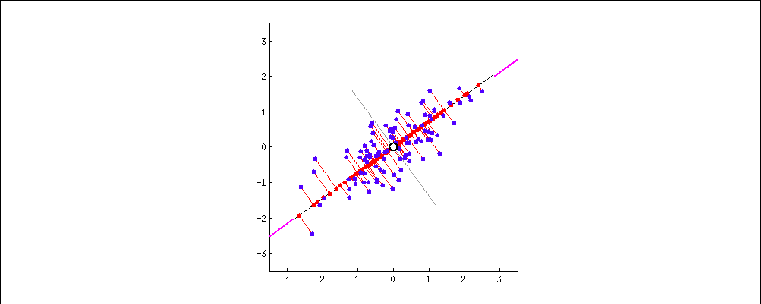
\includegraphics[scale=0.5]{images/PCA_L.png}
		\caption{Prinzipiele Linie}
		\label{PL}
\end{figure}

In der Abbildung \ref{PL} ist die Linie mit der größte Variation und so ist die die erste Prinzipielle Komponente (PK), da sie mit sich die meiste Information trägt. Falls die Variablen dann mit Hilfe dieser PK transformiert werden, wird die meiste Information übertragen. Nachdem die erste Komponente gewählt wird, wird die zweite auf den selben Prinzip gewählt, jedoch wird eine andere Linie gesucht, die dann unabhängig von der erste, meisten eine die Orthogonal zu der Erste liegt. Diese zweite besitzt entsprechend die zweitgrößte Varianz zu den Variablen aus der Datensammlung. Dieser Prozes wiederholt sich bis alle prinzipiellen Komponenten bestimmt sind, oder \emph{p} oft -  genau so oft wie wir Variablen in unsere Kovarianzmatrix haben.

Nun zurück zu den Eigenwerten und -vektoren. Zu Jedem Eigenwert gehört ein Vektor und umgekehrt. Sie Kommen immer in Paare und ihre Anzahl entspricht die dimensionalität der Matrix, wie schon oben erwähnt wurden. Ihre Beziehung in mathematischer Form kann wie folgt dargestellt werden:

\begin{equation}\label{gl1}
	Av = \lambda v,
\end{equation}

wo $\emph{A}$ ist die Matrix, $\emph{v}$ der Eigenvektor und $\lambda$ der zugehörige Eigenwert. Es existiert für eine quadratische Matrix einen Vektor $\emph{v}$ und einen Faktor $\lambda$, sodass bei der Multiplikation der Matrix mit dem Vektor, erhalten wir das gleiche Ergebnis, wie wenn wir den Vektor mit dem Faktor multiplizieren. Es kann die Formel in \ref{gl1} umgeformt werden, um nun die Eigenvektoren und Eigenwerte zu berechnen:

\begin{equation}
	(A - \lambda E).v = 0.
\end{equation}

In der Gleichung enspricht $\emph{E}$ gleich der Einheitsmatrix. Der Eigenvektor ist Lösung der Gleichungssystem. Wir setzte für $\lambda$ den entsprechenden Wert ein und lösen nach v. Jedoch muss der Eigenwert zuerst berechnet werden. Der wird aus der folgenden Formel errechnet:

\begin{equation}
	det(A - \lamda E) = 0
\end{equation}

Wo wir nach den Nullstellen der Determinante suchen. Diese Nullstellen sind die Eingenwerte der Matrix A.

Die Eigenvektoren bestimmen eigentlich die Richtung der Axen mit der meisten Information, oder auch Prinzipielle Komponenten genannt. Die Eingewerte sind die Koeffizienten der Komponente. Je höher der Wert, desto mehr Information wird durch ihre Richtung repräsentiert. Falls die Eigenvektoren nach ihren Eigenwerte absteigend geordnet sind, werden die Ordnung der Prinzipiellen Komponenten bestimmt, sodass die erste Komponente entsprechend diese ist, die den größten Eigenwert besitzt. Als alle Vektoren angeordnet sind, wird einen neuen Vektor aus den zusammengesetzt. Jeder Eigenvektor ist eine Spalte im neuen Vektor. Als nächstes muss die Entscheidung getroffen werden, wie viele prinzipiellen Komponente erhalten werden. Diese Frage hat keine richtige Antwort, in meinem Fall brauche ich nur zwei Komponenten, um die Daten in einem zweidimensionallen Raum darzustellen.


\subsubsection{4. Transformation der Daten}

Im letzten Schritt wird der Prozess abgeschlossen, indem die Ursprungsdaten nach den gefundenen Richtungen ($\emph{Prinzipiellen Komponenten}$), transformiert werden. Die Folgende Formel beschreibt die Operation:

\begin{equation}\label{transPCA}
	T_{L} = V^T_L * Z^T,
\end{equation}  

wo $T_{L}$ die transformierten, $\emph{V}$ enthält die $\emph{L}$ Prinzipiellen Komponenten und $emph{Z}$ beinhaltet den standardisierten Datensatz. Die erhaltene Matrix $\emph{T}$ hat die gewünschte $\emph{L}$ Anzahl an Komponenten. 


QUELLEN:
https://builtin.com/data-science/step-step-explanation-principal-component-analysis

https://royalsocietypublishing.org/doi/10.1098/rsta.2015.0202

https://en.wikipedia.org/wiki/Principal_component_analysis

https://en.wikipedia.org/wiki/Sample_mean_and_covariance

https://www.kaggle.com/jeffd23/visualizing-word-vectors-with-t-sne

https://towardsdatascience.com/visualizing-word-embedding-with-pca-and-t-sne-961a692509f5

https://towardsdatascience.com/visualization-of-word-embedding-vectors-using-gensim-and-pca-8f592a5d3354

https://studyflix.de/mathematik/eigenwert-1635



